\subsection{Red de Centro Comercial}

En este caso la captura se llevó a cabo en una red no controlada, en el shopping Galerías Pacífico, durante aproximadamente 10 minutos.
Debido a que la red no está controlada por nosotros, no conocemos detalles de la naturaleza de los equipos que intercambian información en la misma. Pero conjeturamos que la mayoría podrían ser teléfonos celulares.
\\\\
Vemos a continuación el gráfico que muestra la topología según la captura.

\begin{figure}[ht!]
  \centering
   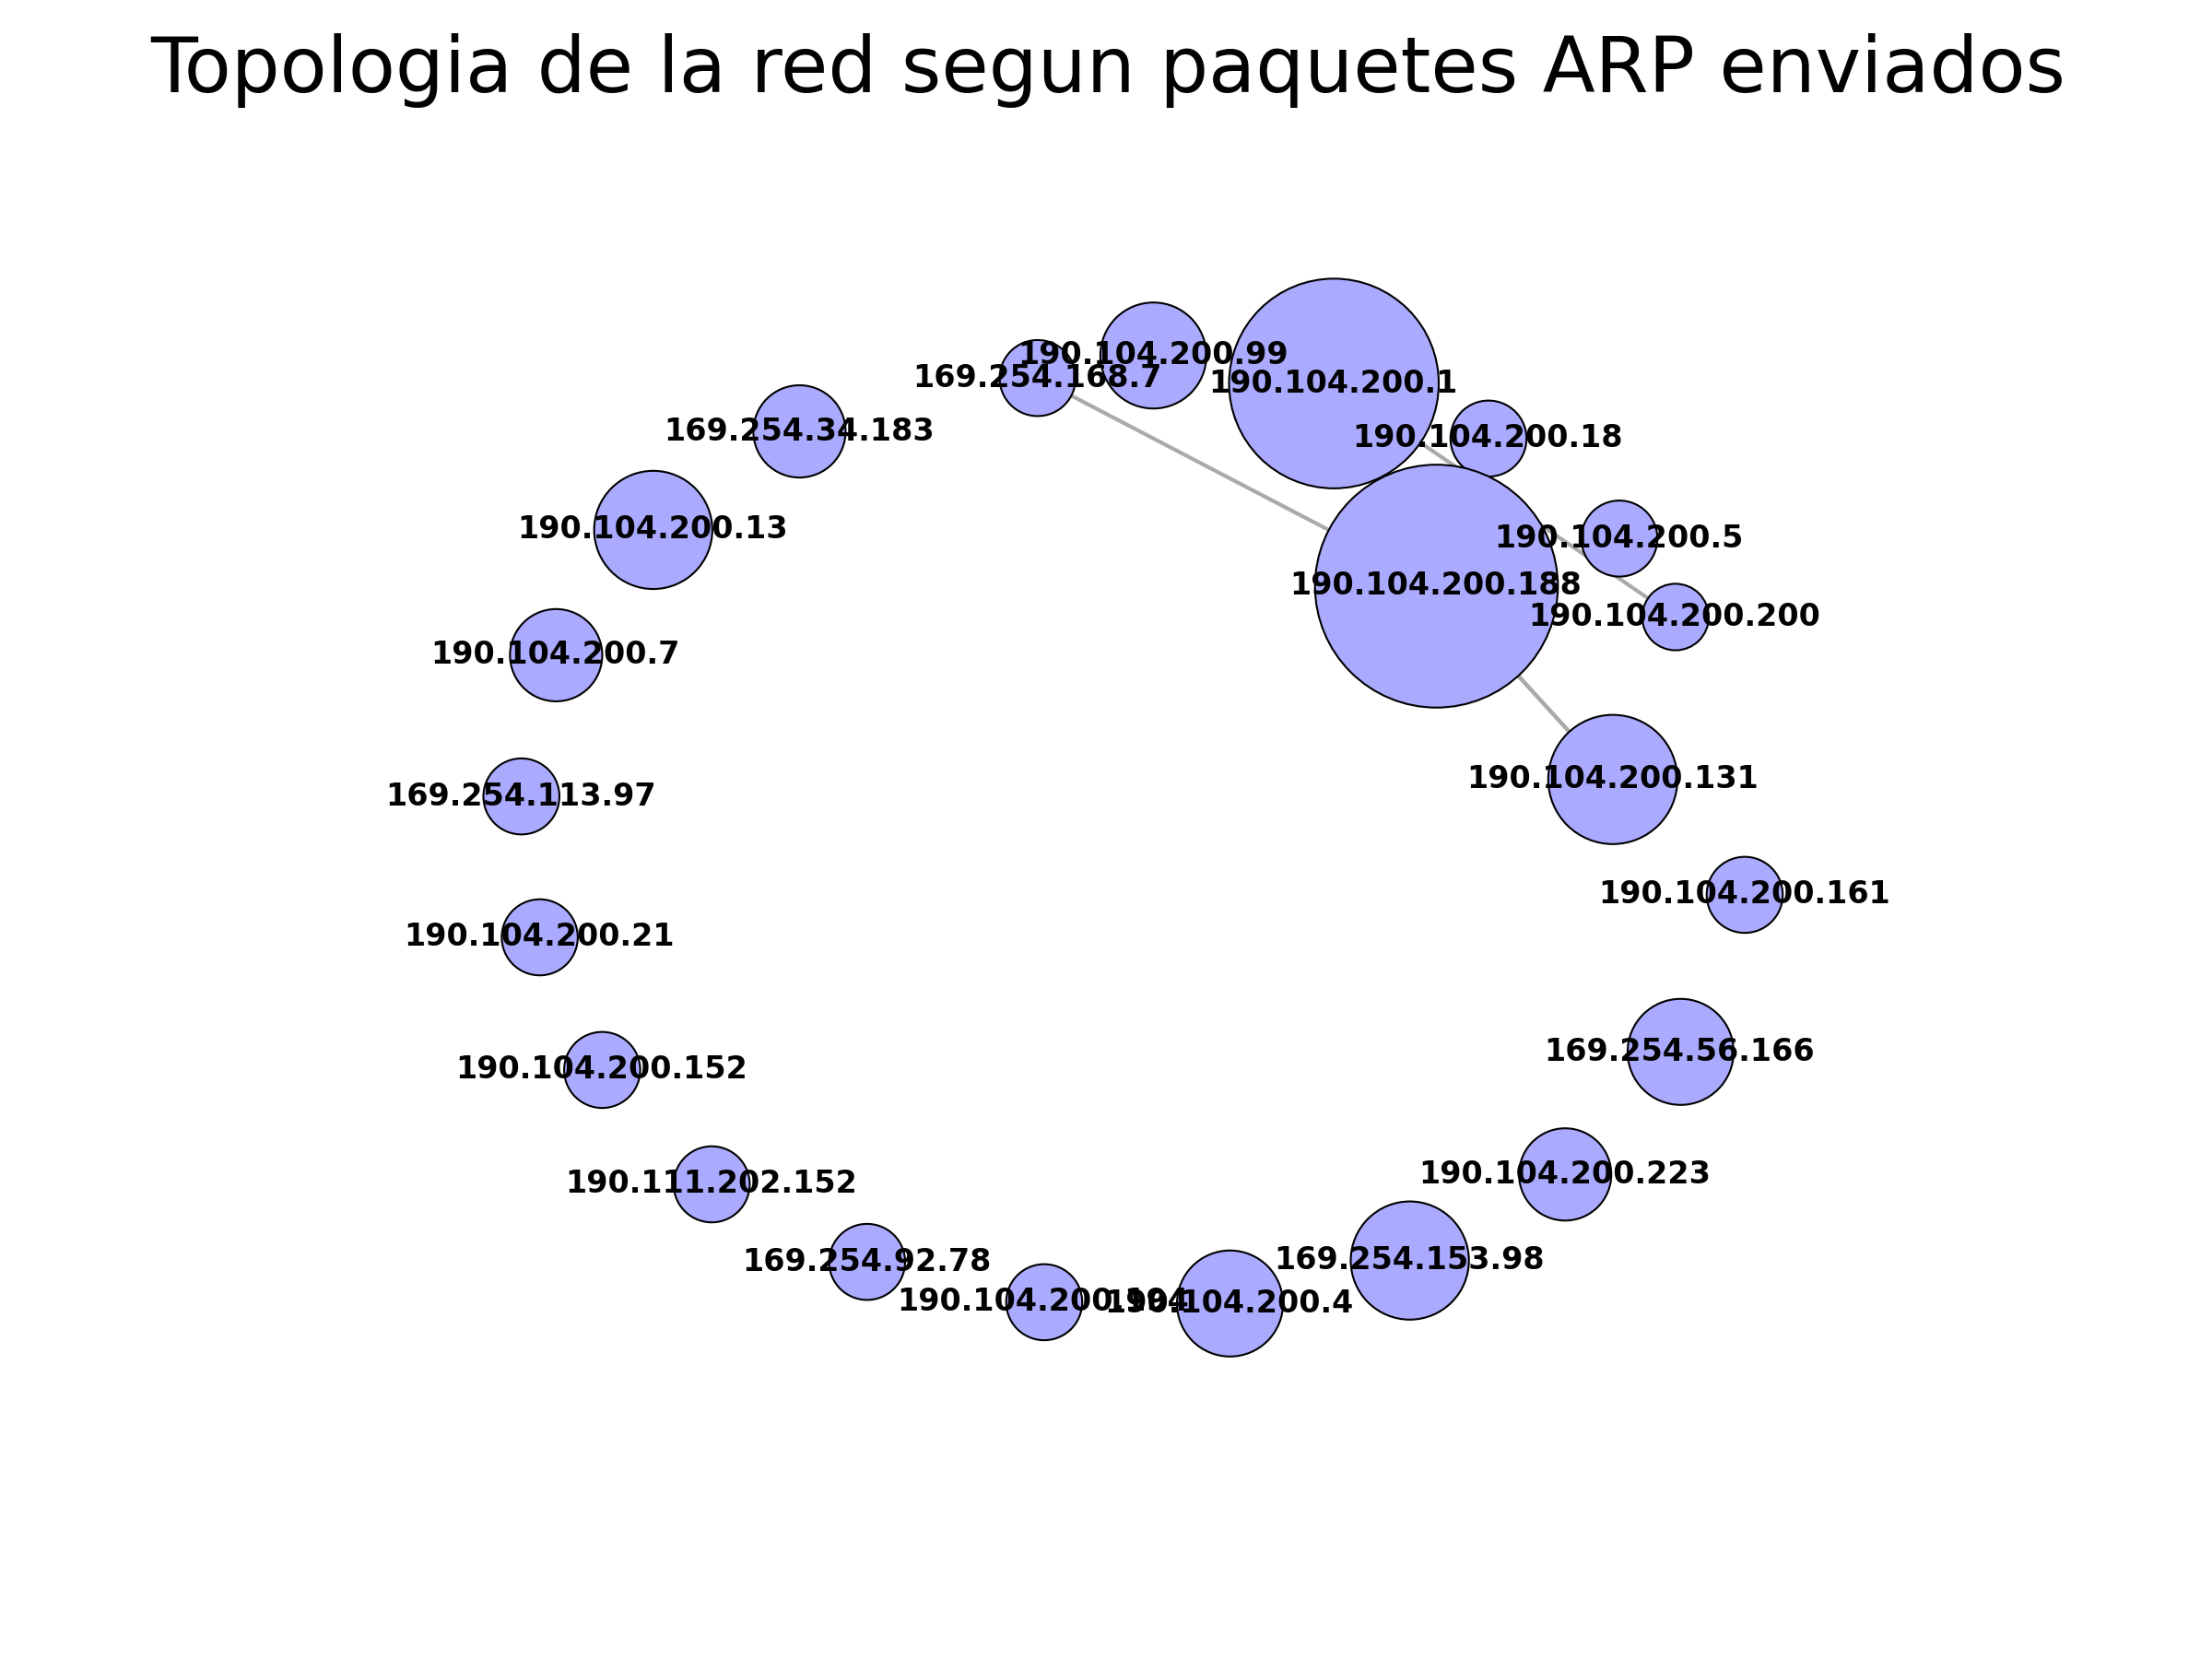
\includegraphics[width=0.7\textwidth]{graficos/shopping_network.png}
  \caption{}
  \label{fig:shopping_network}
\end{figure}

En este diagrama podemos observar que la mayoría de los nodos se encuentran sin un eje que los conecte. Esto se debe a que durante la captura, en general los paquetes ARP tuvieron la misma dirección IP como origen y destino. Según lo que investigamos sobre este comportamiento se debe a una práctica llamada ARP gratuitos. Los paquetes ARP gratuitos contienen en el destino la misma dirección IP que la del origen quien lo envía y la MAC destino es una dirección broadcast. La utilidad de este tipo de paquetes es la de poder detectar conflictos de direcciones IP duplicadas. También se utilizan para informar a los switches, o máquinas,de las MAC de sus interfaces para que actualicen sus tablas sin necesidad de peticiones directas.
\\\\
Observamos a continuación el gráfico de cantidad de información de cada nodo con respecto a la entropía.

\begin{figure}[ht!]
  \centering
   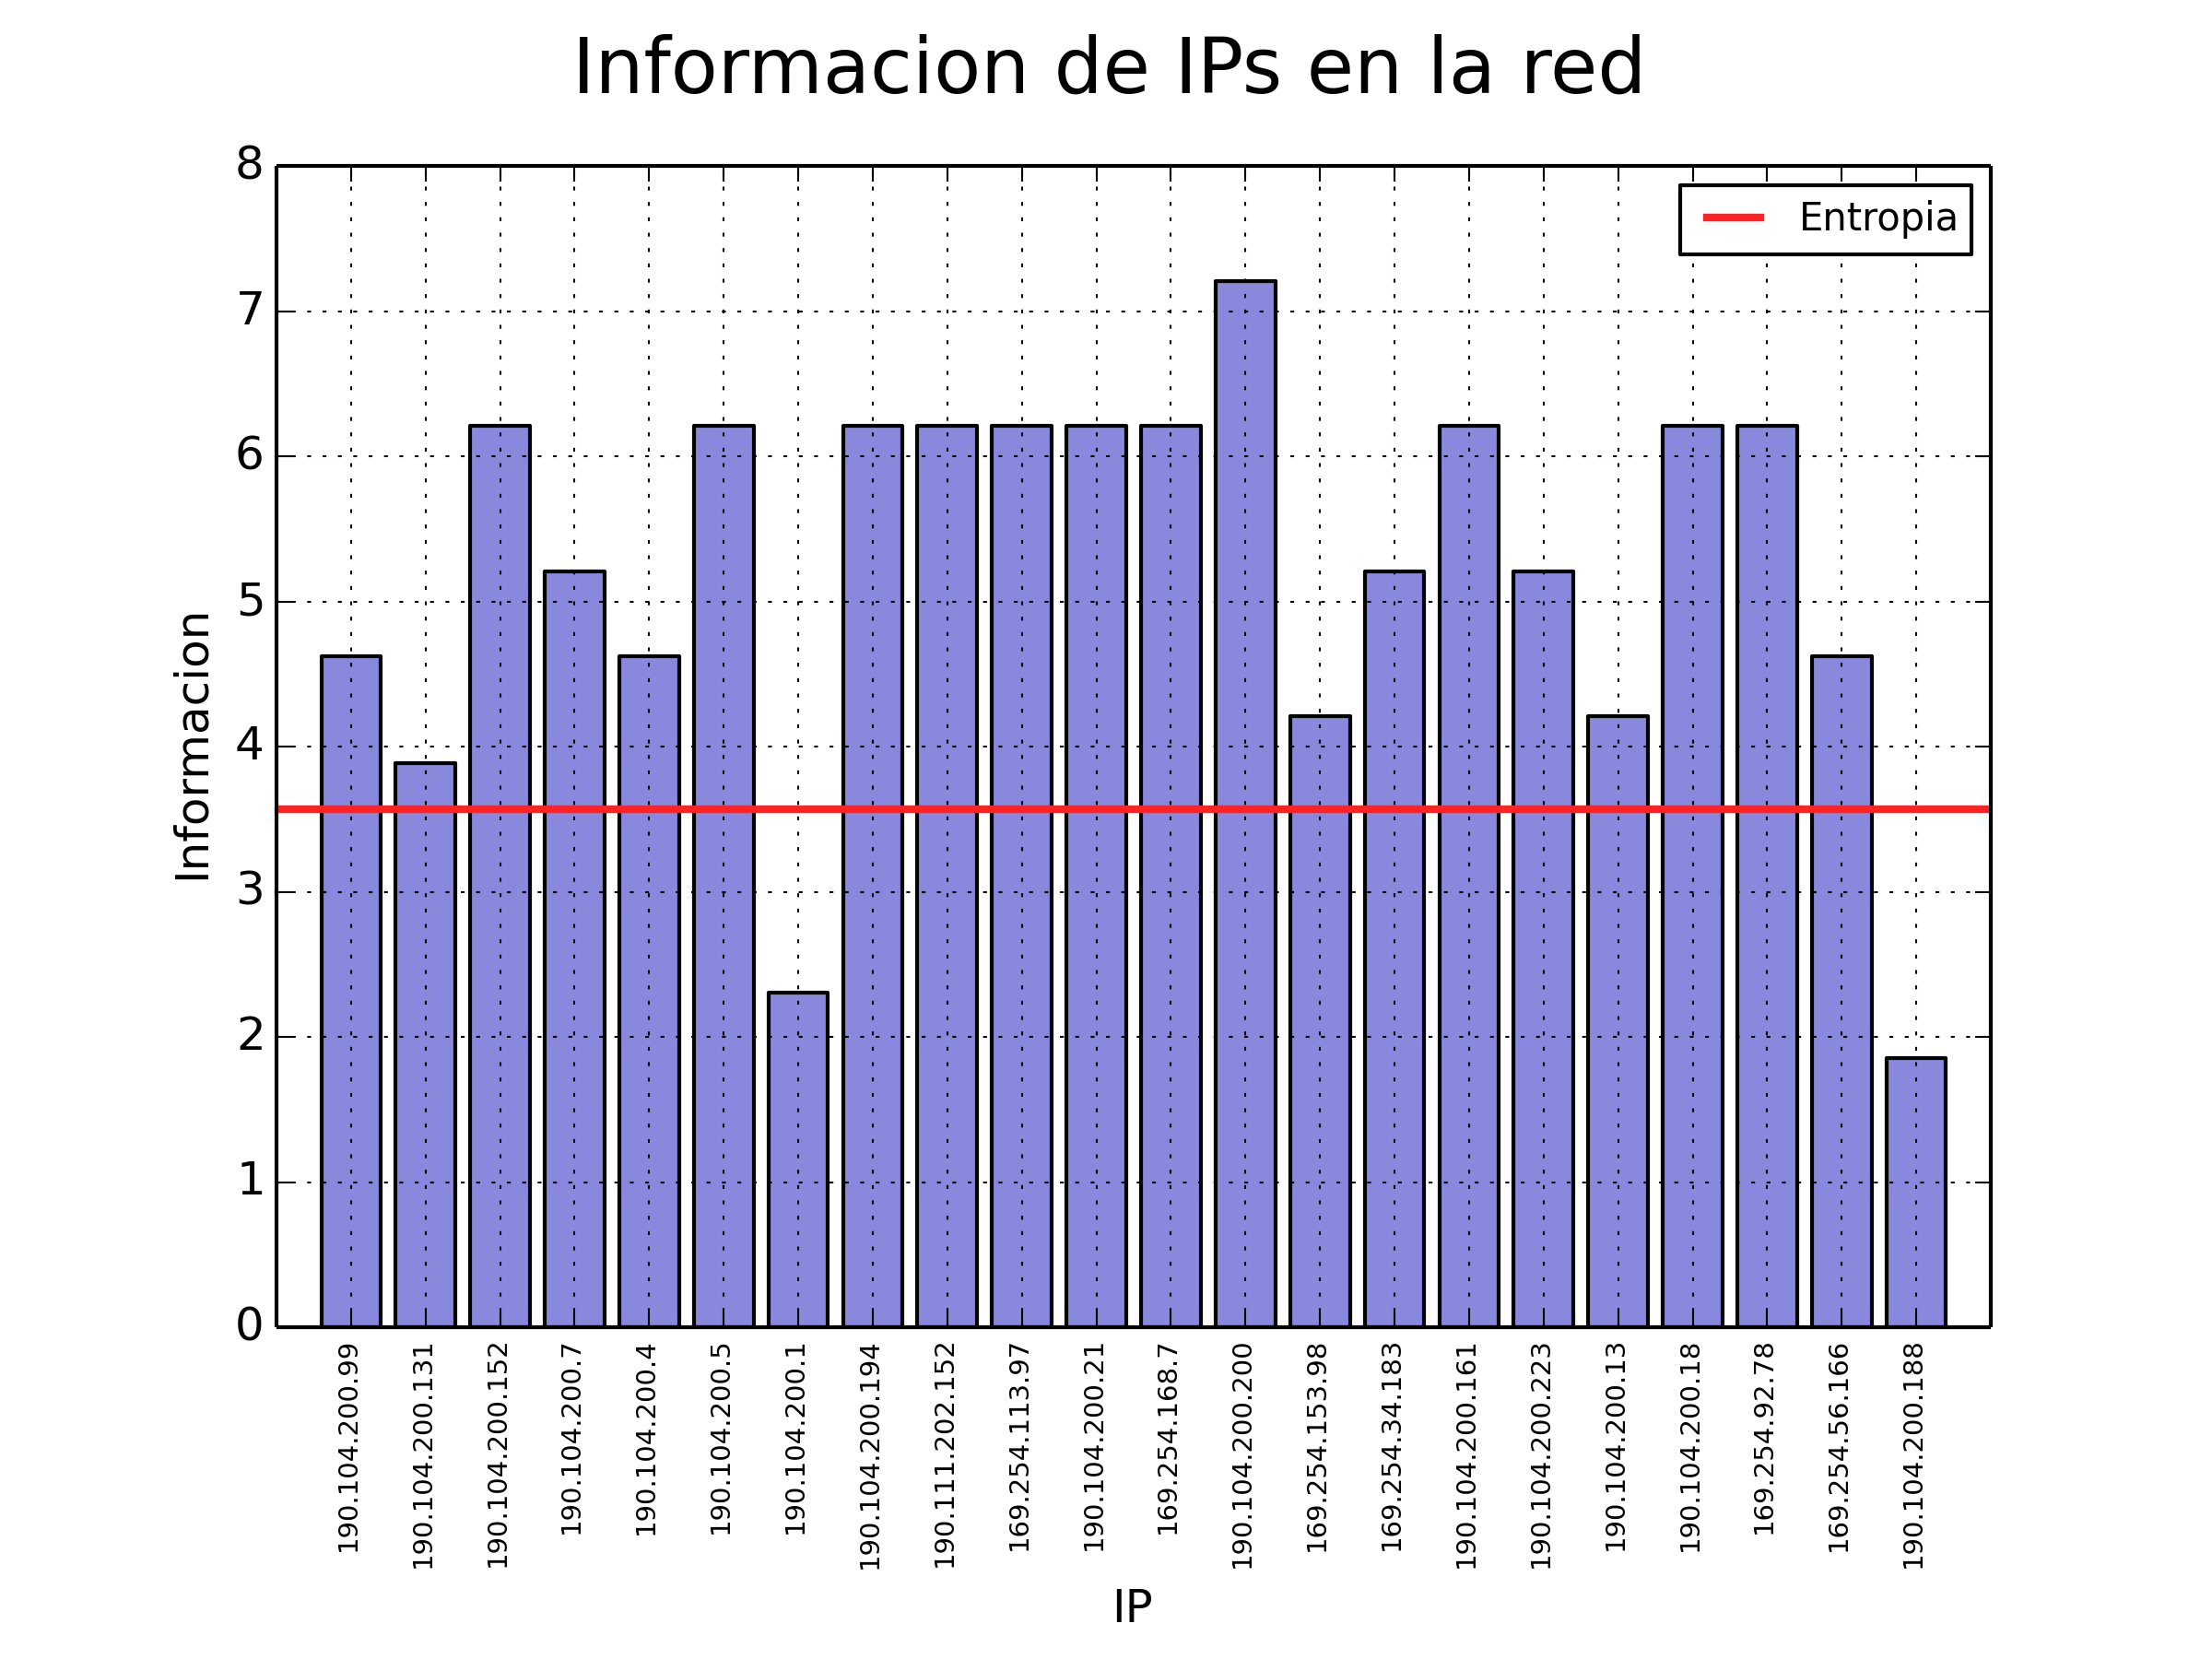
\includegraphics[width=0.7\textwidth]{graficos/shopping_information_bars_arp.png}
  \caption{}
  \label{fig:shopping_information_bars_arp}
\end{figure}

Como podemos observar, hay dos nodos que presentan una cantidad de información que se encuentra por debajo de la entropía. Basándonos en los experimentos analizados anteriormente, inferimos que alguno de estos dos nodos posiblemente sea el router.
\\\\
Vemos el gráfico de la cantidad de información de cada protocolo en comparación con la entropía.

\begin{figure}[ht!]
  \centering
   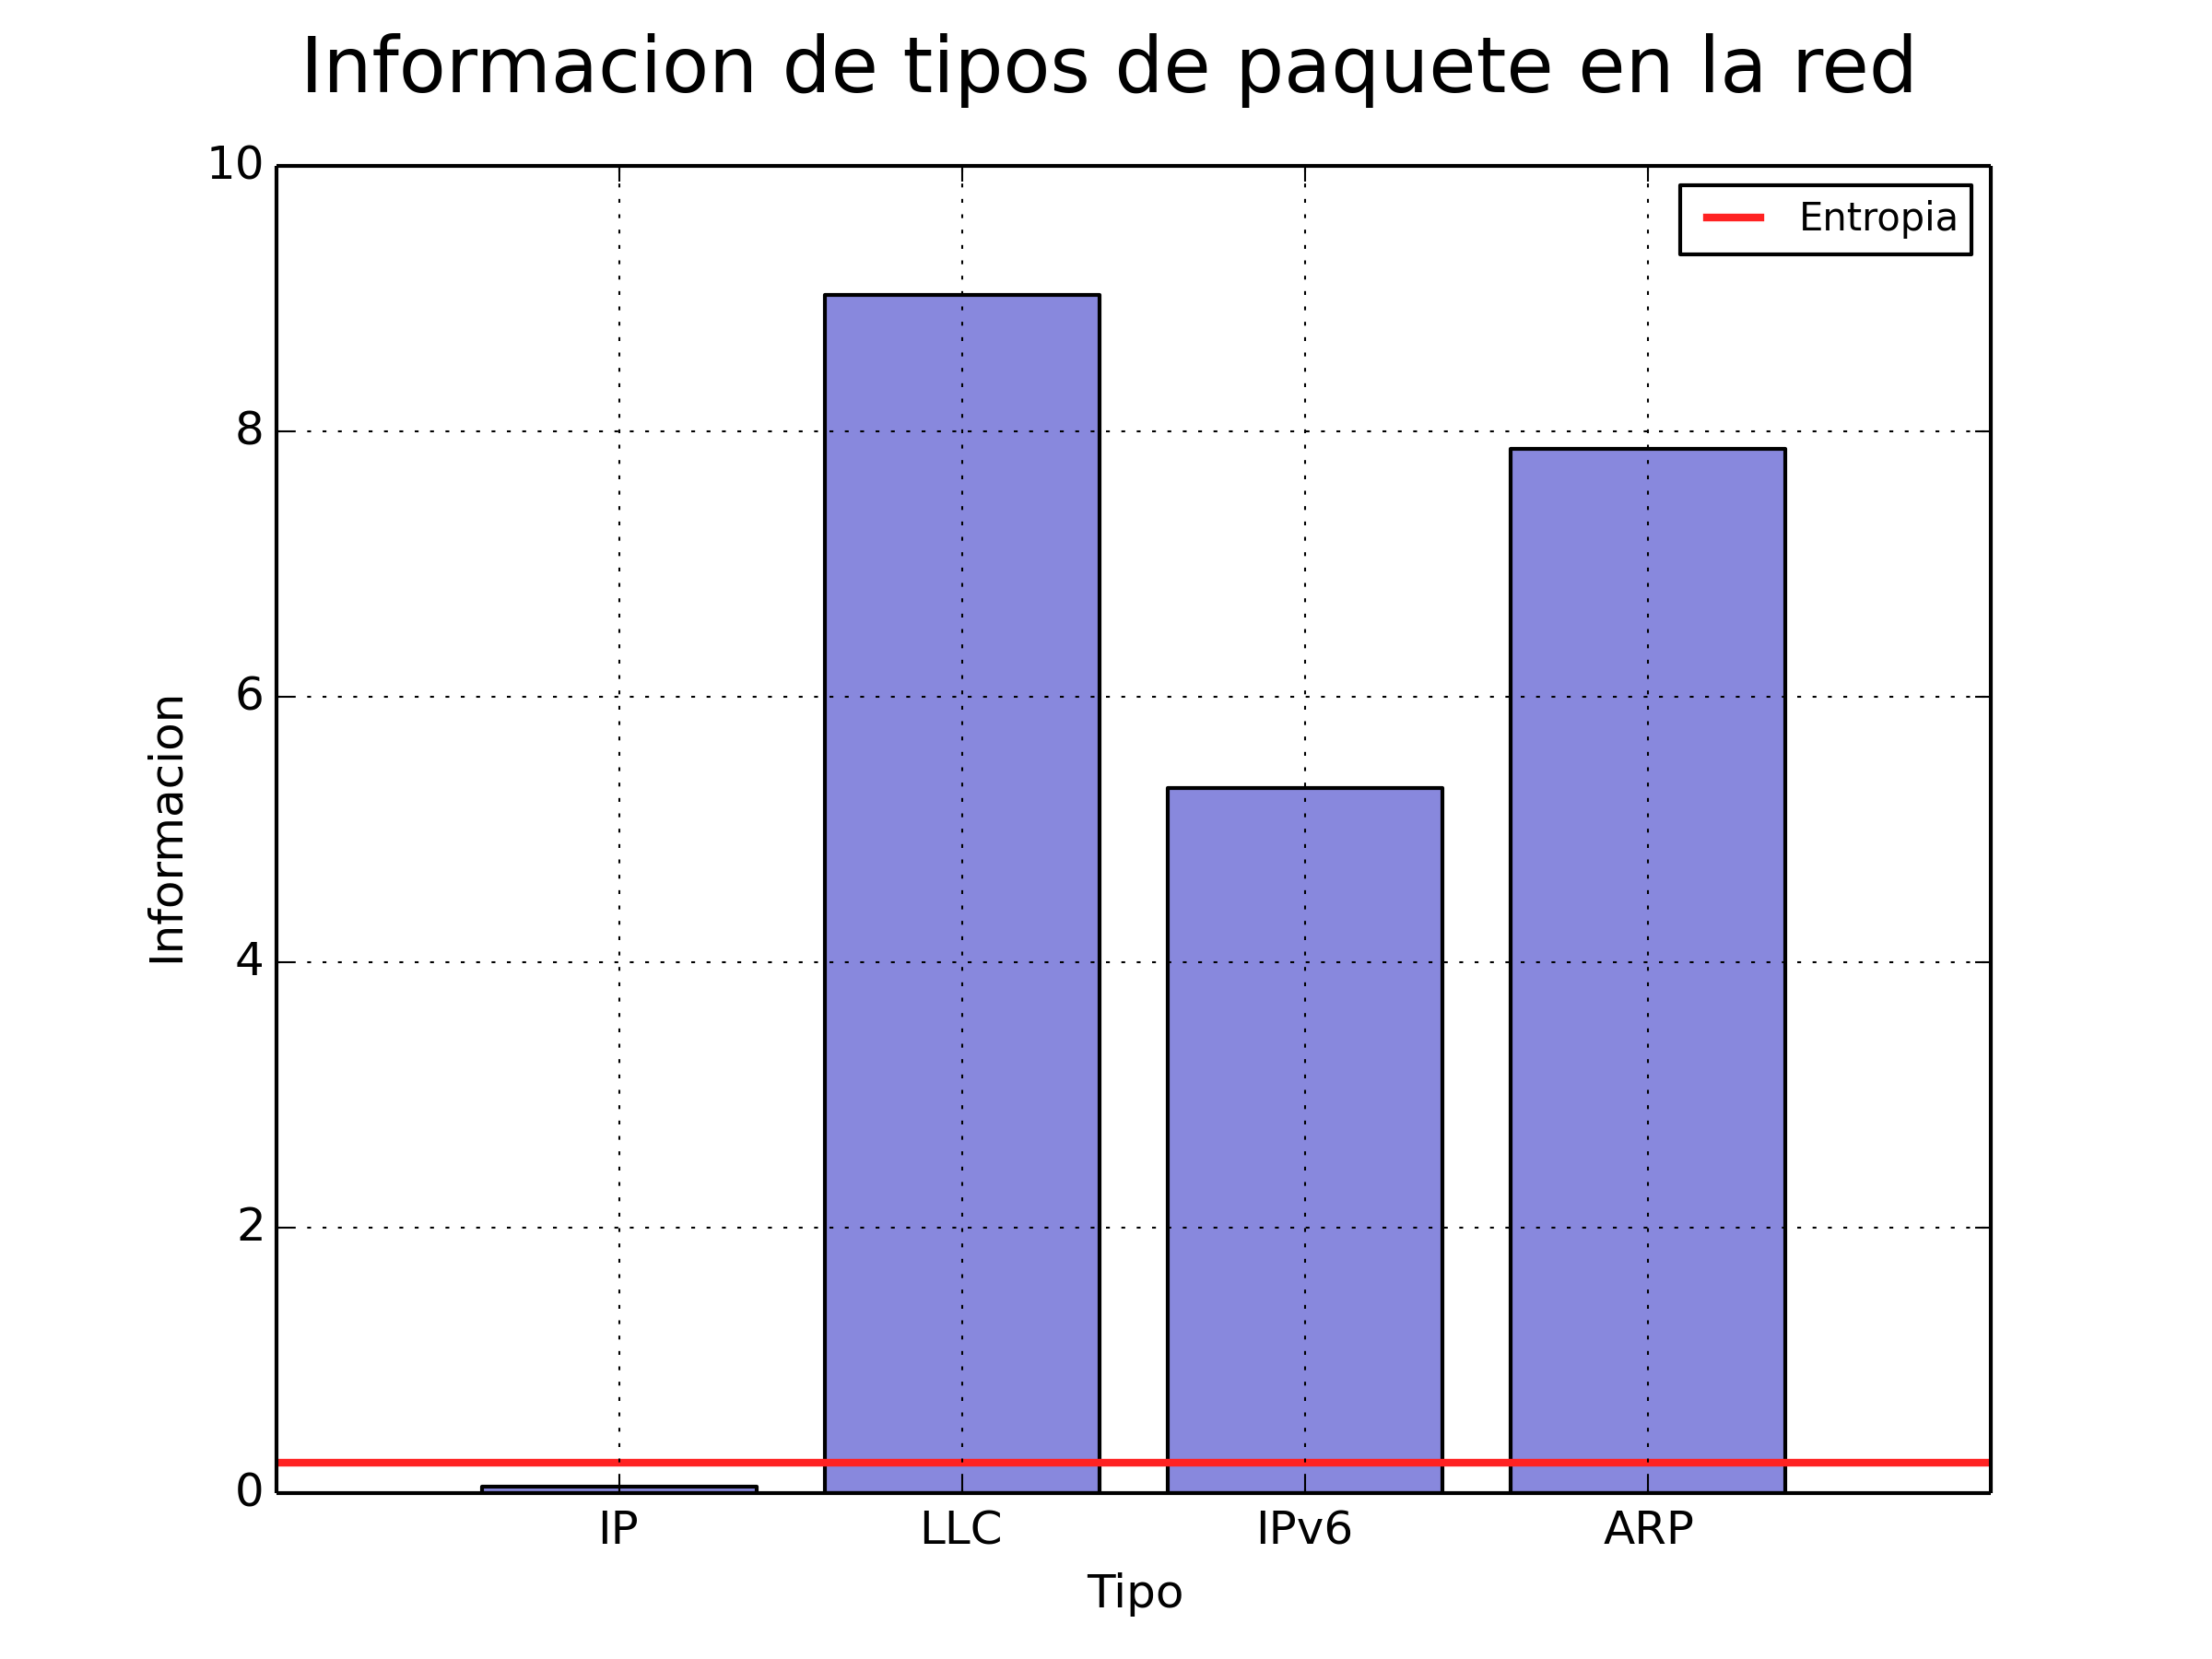
\includegraphics[width=0.7\textwidth]{graficos/shopping_information_bars_type.png}
  \caption{}
  \label{fig:shopping_information_bars_type}
\end{figure}

En este caso los resultados son similares a los obtenidos en los experimentos anteriores. Donde el protocolo IP presenta una cantidad de información por debajo del valor de la entropía. El resto de los protocolos, LLC, IPv6 y ARP, aparecieron con menor frecuencia, aportando mayor cantidad de información.